\documentclass[a4paper,12pt]{article}
\usepackage[12pt]{extsizes}




\usepackage{cmap}					% поиск в PDF
\usepackage{mathtext} 				% русские буквы в формулах
\usepackage[T2A]{fontenc}			% кодировка
\usepackage[utf8]{inputenc}			% кодировка исходного текста
\usepackage[english,russian]{babel}	% локализация и переносы
\usepackage{ulem}                   % зачеркнутый текст
\usepackage{amssymb}			% пакет математики
\usepackage{float}
\usepackage{amsmath}
\usepackage{graphicx}
\DeclareGraphicsExtensions{.png}

%%% Страница
%\usepackage{extsizes} % Возможность сделать 14-й шрифт
\usepackage[left=1cm,right=1cm,top=1cm,bottom=1cm]{geometry} % Простой способ задавать поля
\pagestyle{empty}

\begin{document}


\begin{center}
ФЕДЕРАЛЬНОЕ ГОСУДАРСТВЕННОЕ ОБРАЗОВАТЕЛЬНОЕ БЮДЖЕТНОЕ УЧРЕЖДЕНИЕ ВЫСШЕГО ОБРАЗОВАНИЯ

    \textbf{«ФИНАНСОВЫЙ УНИВЕРСИТЕТ ПРИ ПРАВИТЕЛЬСТВЕ РОССИЙСКОЙ ФЕДЕРАЦИИ»}

Факультет информационных технологий и анализа больших данных

Департамент анализа данных и машинного обучения

\textit{
	\textbf{Дисциплина: «Теория вероятностей и математическая статистика»}}

\textit{Направление подготовки: 01.03.02 «Прикладная математика и информатика»}

\textit{Профиль: «Анализ данных и принятие решений в экономике и финансах»}

\textit{Форма обучения очная, учебный 2020/2021 год, 4 семестр}



\end{center}

\begin{enumerate}

\item


Здесь написанно много всего интересного и полезного о гамма-распределении



\item


$\mathbb{P}(\chi _{20}^{2} > 10.9) =  0.948775$; $\chi _{0.93}^{2} (5) = 1.34721$.



\item


Здесь очень много исчерпывающей информации о выборках из генеральной совокупности и про различные виды выборок



\item


%\folder 2_53d1.png
1) Функция распределения $F_Z(x)$ имеет вид:
$
F_Z(x)=\left\{
\begin{array}{l}
0, x\leqslant 0;\\
\frac{5 x}{3}, 0\leqslant x\leqslant \frac{3}{10}\approx 0,\!3;\\
1 - \frac{3}{20 x}, x\geqslant\frac{3}{10};
\end{array}.
\right.
$
2) Плотность распределения $f_Z(x)$ имеет вид:
$
f_Z(x)=\left\{
\begin{array}{l}
0, x<0;\\
\frac{5}{3}, 0\leqslant x\leqslant \frac{3}{10}\approx 0,\!3;\\
\frac{3}{20 x^{2}}, x\geqslant\frac{3}{10};
\end{array}.
\right.
$


\begin{figure}[H]
    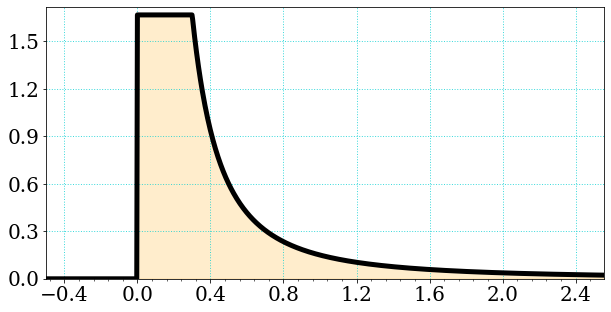
\includegraphics[width=0.9\textwidth]{2_53d1}
\end{figure}


3) вероятность равна:
$
\P(0,\!057\leqslant Z\leqslant 0,\!556)=
0,\!63552.
$



\item


%\folder 2_53d2.png
1) Функция распределения $F_Z(x)$ имеет вид:
$
F_Z(x)=\left\{
\begin{array}{l}
0, x\leqslant 0;\\
x, 0\leqslant x\leqslant \frac{1}{2}\approx 0,\!5;\\
1 - \frac{1}{4 x}, x\geqslant\frac{1}{2};
\end{array}.
\right.
$
2) Плотность распределения $f_Z(x)$ имеет вид:
$
f_Z(x)=\left\{
\begin{array}{l}
0, x<0;\\
1, 0\leqslant x\leqslant \frac{1}{2}\approx 0,\!5;\\
\frac{1}{4 x^{2}}, x\geqslant\frac{1}{2};
\end{array}.
\right.
$


\begin{figure}[H]
    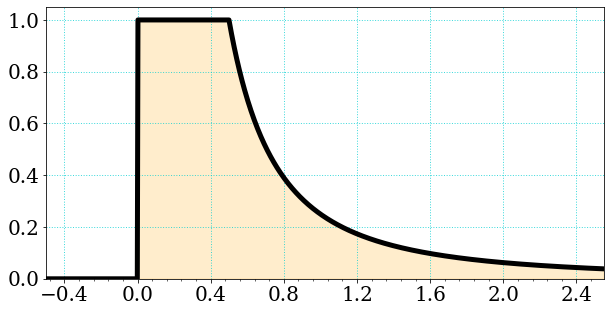
\includegraphics[width=0.9\textwidth]{2_53d2}
\end{figure}


3) вероятность равна:
$
\P(0,\!093\leqslant Z\leqslant 0,\!551)=
0,\!45278.
$



\item


%\folder 2_53d3.png
1) Функция распределения $F_Z(x)$ имеет вид:
$
F_Z(x)=\left\{
\begin{array}{l}
0, x\leqslant 0;\\
\frac{x}{18}, 0\leqslant x\leqslant 9\approx 9,\!0;\\
1 - \frac{9}{2 x}, x\geqslant9;
\end{array}.
\right.
$
2) Плотность распределения $f_Z(x)$ имеет вид:
$
f_Z(x)=\left\{
\begin{array}{l}
0, x<0;\\
\frac{1}{18}, 0\leqslant x\leqslant 9\approx 9,\!0;\\
\frac{9}{2 x^{2}}, x\geqslant9;
\end{array}.
\right.
$


\begin{figure}[H]
    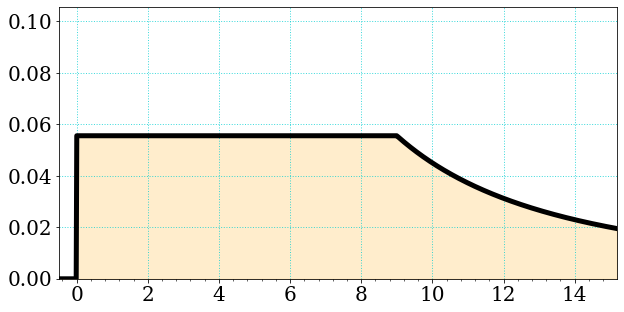
\includegraphics[width=0.9\textwidth]{2_53d3}
\end{figure}


3) вероятность равна:
$
\P(1,\!683\leqslant Z\leqslant 13,\!185)=
0,\!5652.
$



\item


%\folder 2_53d4.png
1) Функция распределения $F_Z(x)$ имеет вид:
$
F_Z(x)=\left\{
\begin{array}{l}
0, x\leqslant 0;\\
2 x, 0\leqslant x\leqslant \frac{1}{4}\approx 0,\!25;\\
1 - \frac{1}{8 x}, x\geqslant\frac{1}{4};
\end{array}.
\right.
$
2) Плотность распределения $f_Z(x)$ имеет вид:
$
f_Z(x)=\left\{
\begin{array}{l}
0, x<0;\\
2, 0\leqslant x\leqslant \frac{1}{4}\approx 0,\!25;\\
\frac{1}{8 x^{2}}, x\geqslant\frac{1}{4};
\end{array}.
\right.
$


\begin{figure}[H]
    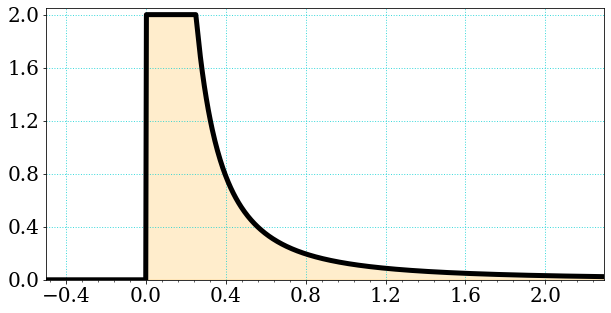
\includegraphics[width=0.9\textwidth]{2_53d4}
\end{figure}


3) вероятность равна:
$
\P(0,\!094\leqslant Z\leqslant 0,\!294)=
0,\!38683.
$



\item


%\folder 2_53d5.png
1) Функция распределения $F_Z(x)$ имеет вид:
$
F_Z(x)=\left\{
\begin{array}{l}
0, x\leqslant 0;\\
\frac{9 x}{20}, 0\leqslant x\leqslant \frac{10}{9}\approx 1,\!111;\\
1 - \frac{5}{9 x}, x\geqslant\frac{10}{9};
\end{array}.
\right.
$
2) Плотность распределения $f_Z(x)$ имеет вид:
$
f_Z(x)=\left\{
\begin{array}{l}
0, x<0;\\
\frac{9}{20}, 0\leqslant x\leqslant \frac{10}{9}\approx 1,\!111;\\
\frac{5}{9 x^{2}}, x\geqslant\frac{10}{9};
\end{array}.
\right.
$


\begin{figure}[H]
    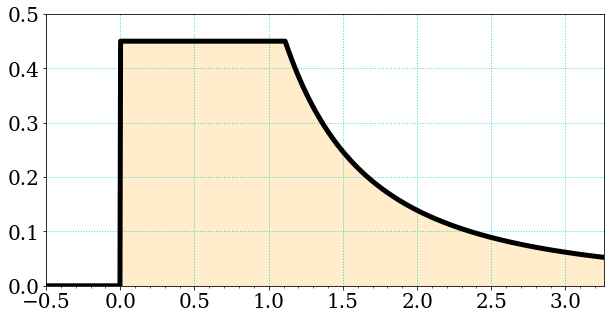
\includegraphics[width=0.9\textwidth]{2_53d5}
\end{figure}


3) вероятность равна:
$
\P(0,\!277\leqslant Z\leqslant 1,\!26)=
0,\!43458.
$



\item


%\folder 2_53d6.png
1) Функция распределения $F_Z(x)$ имеет вид:
$
F_Z(x)=\left\{
\begin{array}{l}
0, x\leqslant 0;\\
\frac{3 x}{8}, 0\leqslant x\leqslant \frac{4}{3}\approx 1,\!333;\\
1 - \frac{2}{3 x}, x\geqslant\frac{4}{3};
\end{array}.
\right.
$
2) Плотность распределения $f_Z(x)$ имеет вид:
$
f_Z(x)=\left\{
\begin{array}{l}
0, x<0;\\
\frac{3}{8}, 0\leqslant x\leqslant \frac{4}{3}\approx 1,\!333;\\
\frac{2}{3 x^{2}}, x\geqslant\frac{4}{3};
\end{array}.
\right.
$


\begin{figure}[H]
    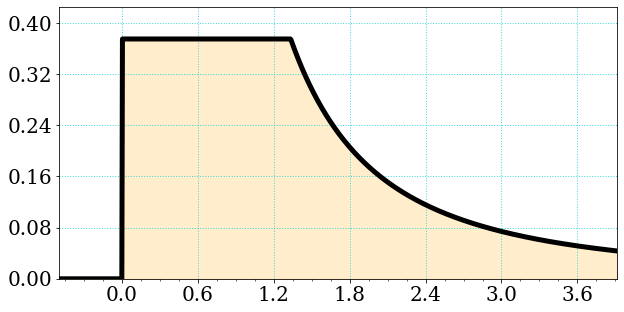
\includegraphics[width=0.9\textwidth]{2_53d6}
\end{figure}


3) вероятность равна:
$
\P(0,\!729\leqslant Z\leqslant 1,\!912)=
0,\!37782.
$



\item


%\folder 2_53d7.png
1) Функция распределения $F_Z(x)$ имеет вид:
$
F_Z(x)=\left\{
\begin{array}{l}
0, x\leqslant 0;\\
3 x, 0\leqslant x\leqslant \frac{1}{6}\approx 0,\!167;\\
1 - \frac{1}{12 x}, x\geqslant\frac{1}{6};
\end{array}.
\right.
$
2) Плотность распределения $f_Z(x)$ имеет вид:
$
f_Z(x)=\left\{
\begin{array}{l}
0, x<0;\\
3, 0\leqslant x\leqslant \frac{1}{6}\approx 0,\!167;\\
\frac{1}{12 x^{2}}, x\geqslant\frac{1}{6};
\end{array}.
\right.
$


\begin{figure}[H]
    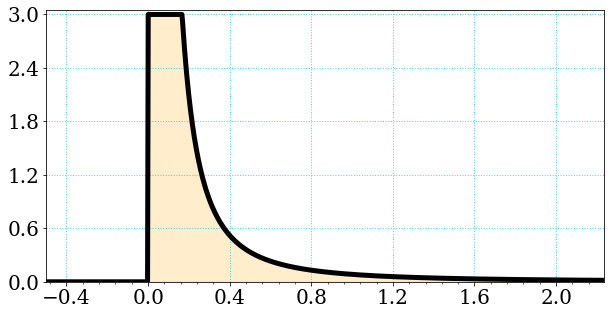
\includegraphics[width=0.9\textwidth]{2_53d7}
\end{figure}


3) вероятность равна:
$
\P(0,\!087\leqslant Z\leqslant 0,\!235)=
0,\!38564.
$



\item


%\folder 2_53d8.png
1) Функция распределения $F_Z(x)$ имеет вид:
$
F_Z(x)=\left\{
\begin{array}{l}
0, x\leqslant 0;\\
\frac{3 x}{16}, 0\leqslant x\leqslant \frac{8}{3}\approx 2,\!667;\\
1 - \frac{4}{3 x}, x\geqslant\frac{8}{3};
\end{array}.
\right.
$
2) Плотность распределения $f_Z(x)$ имеет вид:
$
f_Z(x)=\left\{
\begin{array}{l}
0, x<0;\\
\frac{3}{16}, 0\leqslant x\leqslant \frac{8}{3}\approx 2,\!667;\\
\frac{4}{3 x^{2}}, x\geqslant\frac{8}{3};
\end{array}.
\right.
$


\begin{figure}[H]
    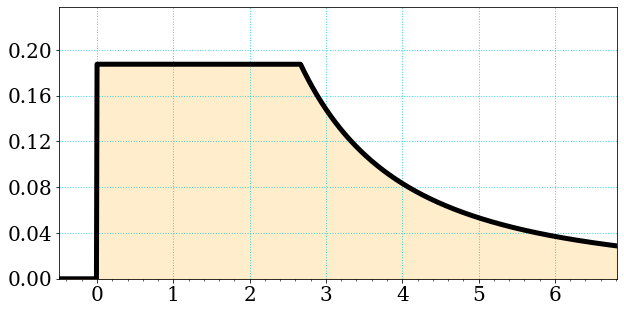
\includegraphics[width=0.9\textwidth]{2_53d8}
\end{figure}


3) вероятность равна:
$
\P(2,\!475\leqslant Z\leqslant 4,\!811)=
0,\!25884.
$



\item


%\folder 2_53d9.png
1) Функция распределения $F_Z(x)$ имеет вид:
$
F_Z(x)=\left\{
\begin{array}{l}
0, x\leqslant 0;\\
\frac{x}{4}, 0\leqslant x\leqslant 2\approx 2,\!0;\\
1 - \frac{1}{x}, x\geqslant2;
\end{array}.
\right.
$
2) Плотность распределения $f_Z(x)$ имеет вид:
$
f_Z(x)=\left\{
\begin{array}{l}
0, x<0;\\
\frac{1}{4}, 0\leqslant x\leqslant 2\approx 2,\!0;\\
\frac{1}{x^{2}}, x\geqslant2;
\end{array}.
\right.
$


\begin{figure}[H]
    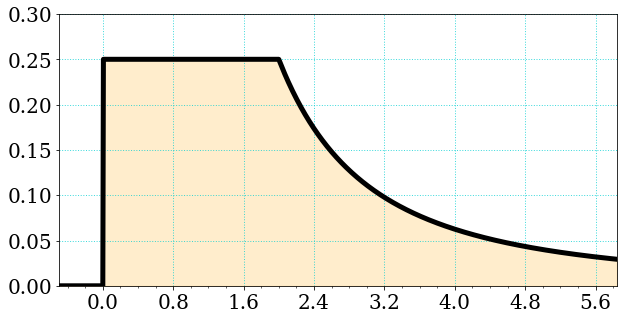
\includegraphics[width=0.9\textwidth]{2_53d9}
\end{figure}


3) вероятность равна:
$
\P(0,\!588\leqslant Z\leqslant 3,\!842)=
0,\!59272.
$



\item


%\folder 2_53d10.png
1) Функция распределения $F_Z(x)$ имеет вид:
$
F_Z(x)=\left\{
\begin{array}{l}
0, x\leqslant 0;\\
\frac{x}{16}, 0\leqslant x\leqslant 8\approx 8,\!0;\\
1 - \frac{4}{x}, x\geqslant8;
\end{array}.
\right.
$
2) Плотность распределения $f_Z(x)$ имеет вид:
$
f_Z(x)=\left\{
\begin{array}{l}
0, x<0;\\
\frac{1}{16}, 0\leqslant x\leqslant 8\approx 8,\!0;\\
\frac{4}{x^{2}}, x\geqslant8;
\end{array}.
\right.
$


\begin{figure}[H]
    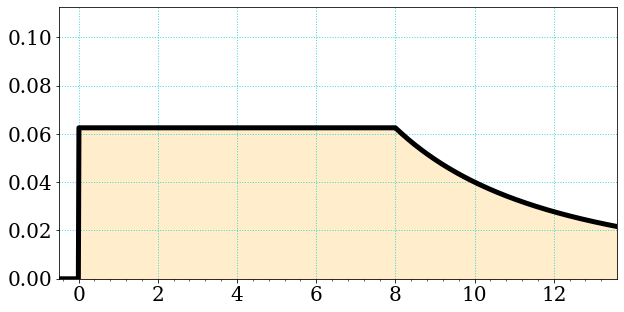
\includegraphics[width=0.9\textwidth]{2_53d10}
\end{figure}


3) вероятность равна:
$
\P(0,\!16\leqslant Z\leqslant 11,\!592)=
0,\!64493.
$



\item


%\folder 2_53d11.png
1) Функция распределения $F_Z(x)$ имеет вид:
$
F_Z(x)=\left\{
\begin{array}{l}
0, x\leqslant 0;\\
\frac{2 x}{3}, 0\leqslant x\leqslant \frac{3}{4}\approx 0,\!75;\\
1 - \frac{3}{8 x}, x\geqslant\frac{3}{4};
\end{array}.
\right.
$
2) Плотность распределения $f_Z(x)$ имеет вид:
$
f_Z(x)=\left\{
\begin{array}{l}
0, x<0;\\
\frac{2}{3}, 0\leqslant x\leqslant \frac{3}{4}\approx 0,\!75;\\
\frac{3}{8 x^{2}}, x\geqslant\frac{3}{4};
\end{array}.
\right.
$


\begin{figure}[H]
    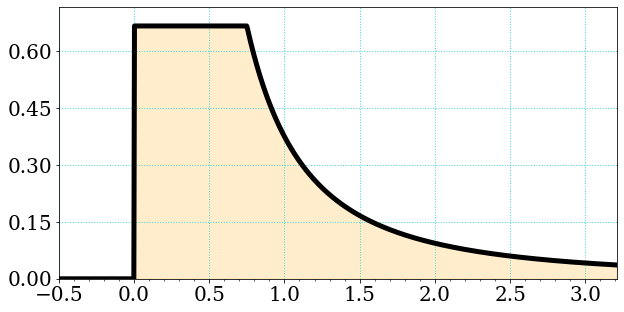
\includegraphics[width=0.9\textwidth]{2_53d11}
\end{figure}


3) вероятность равна:
$
\P(0,\!182\leqslant Z\leqslant 1,\!21)=
0,\!56852.
$



\item


%\folder 2_53d12.png
1) Функция распределения $F_Z(x)$ имеет вид:
$
F_Z(x)=\left\{
\begin{array}{l}
0, x\leqslant 0;\\
\frac{2 x}{7}, 0\leqslant x\leqslant \frac{7}{4}\approx 1,\!75;\\
1 - \frac{7}{8 x}, x\geqslant\frac{7}{4};
\end{array}.
\right.
$
2) Плотность распределения $f_Z(x)$ имеет вид:
$
f_Z(x)=\left\{
\begin{array}{l}
0, x<0;\\
\frac{2}{7}, 0\leqslant x\leqslant \frac{7}{4}\approx 1,\!75;\\
\frac{7}{8 x^{2}}, x\geqslant\frac{7}{4};
\end{array}.
\right.
$


\begin{figure}[H]
    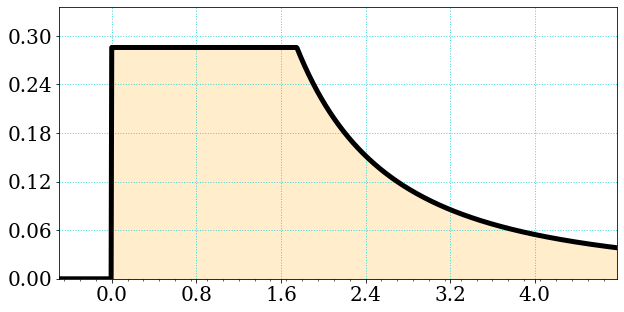
\includegraphics[width=0.9\textwidth]{2_53d12}
\end{figure}


3) вероятность равна:
$
\P(0,\!035\leqslant Z\leqslant 2,\!775)=
0,\!67474.
$



\item


%\folder 2_53d13.png
1) Функция распределения $F_Z(x)$ имеет вид:
$
F_Z(x)=\left\{
\begin{array}{l}
0, x\leqslant 0;\\
\frac{x}{20}, 0\leqslant x\leqslant 10\approx 10,\!0;\\
1 - \frac{5}{x}, x\geqslant10;
\end{array}.
\right.
$
2) Плотность распределения $f_Z(x)$ имеет вид:
$
f_Z(x)=\left\{
\begin{array}{l}
0, x<0;\\
\frac{1}{20}, 0\leqslant x\leqslant 10\approx 10,\!0;\\
\frac{5}{x^{2}}, x\geqslant10;
\end{array}.
\right.
$


\begin{figure}[H]
    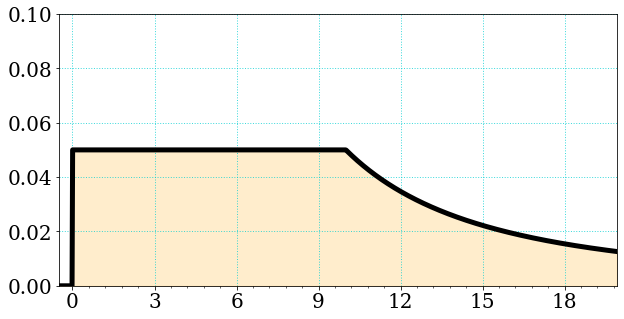
\includegraphics[width=0.9\textwidth]{2_53d13}
\end{figure}


3) вероятность равна:
$
\P(2,\!96\leqslant Z\leqslant 17,\!91)=
0,\!57283.
$



\item


%\folder 2_53d14.png
1) Функция распределения $F_Z(x)$ имеет вид:
$
F_Z(x)=\left\{
\begin{array}{l}
0, x\leqslant 0;\\
\frac{5 x}{9}, 0\leqslant x\leqslant \frac{9}{10}\approx 0,\!9;\\
1 - \frac{9}{20 x}, x\geqslant\frac{9}{10};
\end{array}.
\right.
$
2) Плотность распределения $f_Z(x)$ имеет вид:
$
f_Z(x)=\left\{
\begin{array}{l}
0, x<0;\\
\frac{5}{9}, 0\leqslant x\leqslant \frac{9}{10}\approx 0,\!9;\\
\frac{9}{20 x^{2}}, x\geqslant\frac{9}{10};
\end{array}.
\right.
$


\begin{figure}[H]
    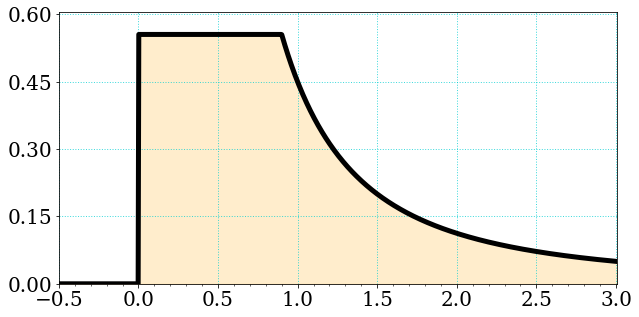
\includegraphics[width=0.9\textwidth]{2_53d14}
\end{figure}


3) вероятность равна:
$
\P(0,\!719\leqslant Z\leqslant 1,\!005)=
0,\!15287.
$



\item


%\folder 2_53d15.png
1) Функция распределения $F_Z(x)$ имеет вид:
$
F_Z(x)=\left\{
\begin{array}{l}
0, x\leqslant 0;\\
\frac{x}{7}, 0\leqslant x\leqslant \frac{7}{2}\approx 3,\!5;\\
1 - \frac{7}{4 x}, x\geqslant\frac{7}{2};
\end{array}.
\right.
$
2) Плотность распределения $f_Z(x)$ имеет вид:
$
f_Z(x)=\left\{
\begin{array}{l}
0, x<0;\\
\frac{1}{7}, 0\leqslant x\leqslant \frac{7}{2}\approx 3,\!5;\\
\frac{7}{4 x^{2}}, x\geqslant\frac{7}{2};
\end{array}.
\right.
$


\begin{figure}[H]
    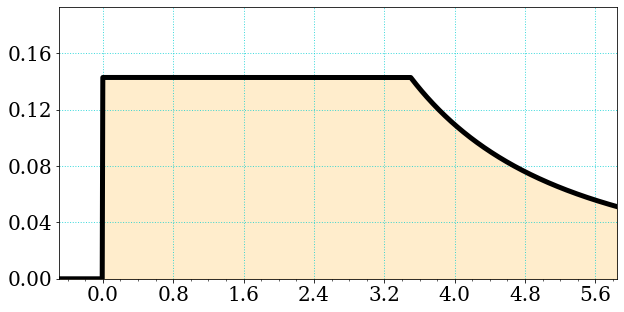
\includegraphics[width=0.9\textwidth]{2_53d15}
\end{figure}


3) вероятность равна:
$
\P(2,\!019\leqslant Z\leqslant 3,\!843)=
0,\!25613.
$



\item


%\folder 2_53d16.png
1) Функция распределения $F_Z(x)$ имеет вид:
$
F_Z(x)=\left\{
\begin{array}{l}
0, x\leqslant 0;\\
\frac{x}{4}, 0\leqslant x\leqslant 2\approx 2,\!0;\\
1 - \frac{1}{x}, x\geqslant2;
\end{array}.
\right.
$
2) Плотность распределения $f_Z(x)$ имеет вид:
$
f_Z(x)=\left\{
\begin{array}{l}
0, x<0;\\
\frac{1}{4}, 0\leqslant x\leqslant 2\approx 2,\!0;\\
\frac{1}{x^{2}}, x\geqslant2;
\end{array}.
\right.
$


\begin{figure}[H]
    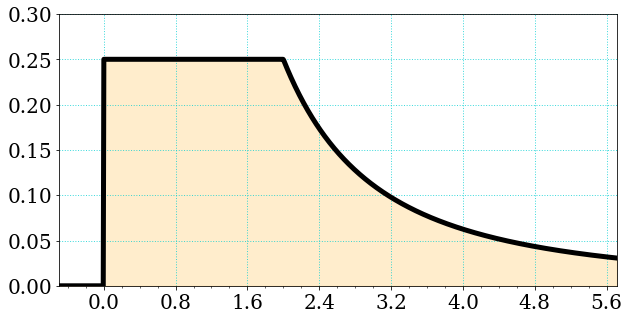
\includegraphics[width=0.9\textwidth]{2_53d16}
\end{figure}


3) вероятность равна:
$
\P(0,\!1\leqslant Z\leqslant 3,\!714)=
0,\!70575.
$



\item


%\folder 2_53d17.png
1) Функция распределения $F_Z(x)$ имеет вид:
$
F_Z(x)=\left\{
\begin{array}{l}
0, x\leqslant 0;\\
\frac{x}{3}, 0\leqslant x\leqslant \frac{3}{2}\approx 1,\!5;\\
1 - \frac{3}{4 x}, x\geqslant\frac{3}{2};
\end{array}.
\right.
$
2) Плотность распределения $f_Z(x)$ имеет вид:
$
f_Z(x)=\left\{
\begin{array}{l}
0, x<0;\\
\frac{1}{3}, 0\leqslant x\leqslant \frac{3}{2}\approx 1,\!5;\\
\frac{3}{4 x^{2}}, x\geqslant\frac{3}{2};
\end{array}.
\right.
$


\begin{figure}[H]
    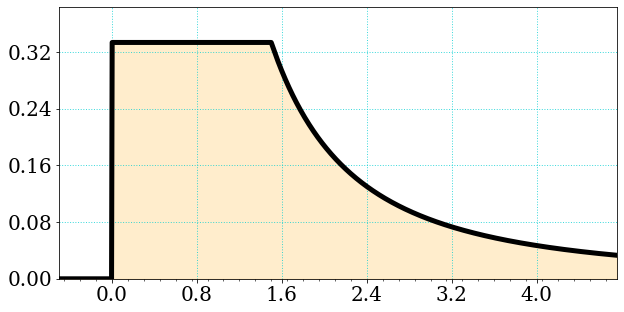
\includegraphics[width=0.9\textwidth]{2_53d17}
\end{figure}


3) вероятность равна:
$
\P(1,\!179\leqslant Z\leqslant 2,\!754)=
0,\!33467.
$



\item


%\folder 2_53d18.png
1) Функция распределения $F_Z(x)$ имеет вид:
$
F_Z(x)=\left\{
\begin{array}{l}
0, x\leqslant 0;\\
\frac{7 x}{6}, 0\leqslant x\leqslant \frac{3}{7}\approx 0,\!429;\\
1 - \frac{3}{14 x}, x\geqslant\frac{3}{7};
\end{array}.
\right.
$
2) Плотность распределения $f_Z(x)$ имеет вид:
$
f_Z(x)=\left\{
\begin{array}{l}
0, x<0;\\
\frac{7}{6}, 0\leqslant x\leqslant \frac{3}{7}\approx 0,\!429;\\
\frac{3}{14 x^{2}}, x\geqslant\frac{3}{7};
\end{array}.
\right.
$


\begin{figure}[H]
    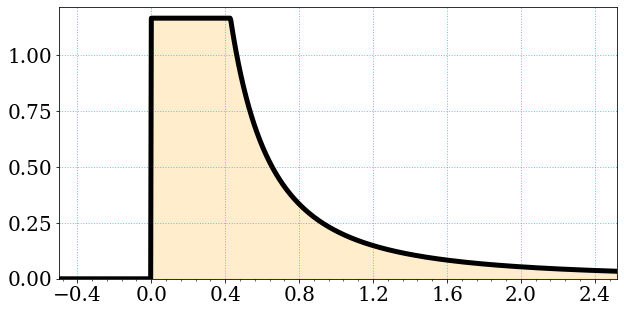
\includegraphics[width=0.9\textwidth]{2_53d18}
\end{figure}


3) вероятность равна:
$
\P(0,\!006\leqslant Z\leqslant 0,\!519)=
0,\!57962.
$



\item


%\folder 2_53d19.png
1) Функция распределения $F_Z(x)$ имеет вид:
$
F_Z(x)=\left\{
\begin{array}{l}
0, x\leqslant 0;\\
\frac{3 x}{2}, 0\leqslant x\leqslant \frac{1}{3}\approx 0,\!333;\\
1 - \frac{1}{6 x}, x\geqslant\frac{1}{3};
\end{array}.
\right.
$
2) Плотность распределения $f_Z(x)$ имеет вид:
$
f_Z(x)=\left\{
\begin{array}{l}
0, x<0;\\
\frac{3}{2}, 0\leqslant x\leqslant \frac{1}{3}\approx 0,\!333;\\
\frac{1}{6 x^{2}}, x\geqslant\frac{1}{3};
\end{array}.
\right.
$


\begin{figure}[H]
    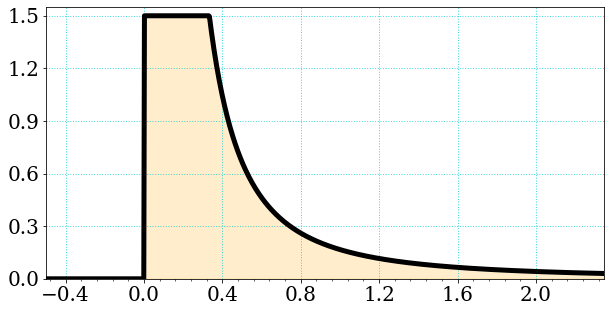
\includegraphics[width=0.9\textwidth]{2_53d19}
\end{figure}


3) вероятность равна:
$
\P(0,\!059\leqslant Z\leqslant 0,\!348)=
0,\!43307.
$



\item


%\folder 2_53d20.png
1) Функция распределения $F_Z(x)$ имеет вид:
$
F_Z(x)=\left\{
\begin{array}{l}
0, x\leqslant 0;\\
\frac{x}{6}, 0\leqslant x\leqslant 3\approx 3,\!0;\\
1 - \frac{3}{2 x}, x\geqslant3;
\end{array}.
\right.
$
2) Плотность распределения $f_Z(x)$ имеет вид:
$
f_Z(x)=\left\{
\begin{array}{l}
0, x<0;\\
\frac{1}{6}, 0\leqslant x\leqslant 3\approx 3,\!0;\\
\frac{3}{2 x^{2}}, x\geqslant3;
\end{array}.
\right.
$


\begin{figure}[H]
    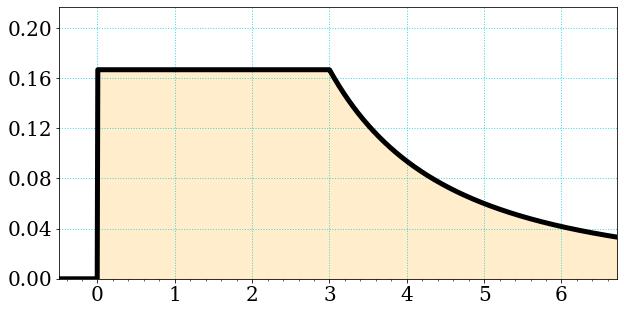
\includegraphics[width=0.9\textwidth]{2_53d20}
\end{figure}


3) вероятность равна:
$
\P(2,\!532\leqslant Z\leqslant 4,\!716)=
0,\!25993.
$



\item


%\folder 2_53d21.png
1) Функция распределения $F_Z(x)$ имеет вид:
$
F_Z(x)=\left\{
\begin{array}{l}
0, x\leqslant 0;\\
\frac{x}{6}, 0\leqslant x\leqslant 3\approx 3,\!0;\\
1 - \frac{3}{2 x}, x\geqslant3;
\end{array}.
\right.
$
2) Плотность распределения $f_Z(x)$ имеет вид:
$
f_Z(x)=\left\{
\begin{array}{l}
0, x<0;\\
\frac{1}{6}, 0\leqslant x\leqslant 3\approx 3,\!0;\\
\frac{3}{2 x^{2}}, x\geqslant3;
\end{array}.
\right.
$


\begin{figure}[H]
    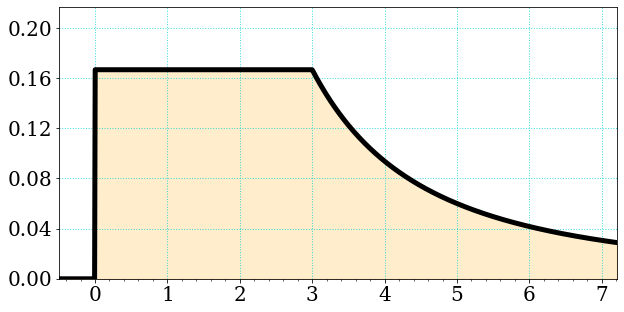
\includegraphics[width=0.9\textwidth]{2_53d21}
\end{figure}


3) вероятность равна:
$
\P(0,\!039\leqslant Z\leqslant 5,\!208)=
0,\!70548.
$



\item


%\folder 2_53d22.png
1) Функция распределения $F_Z(x)$ имеет вид:
$
F_Z(x)=\left\{
\begin{array}{l}
0, x\leqslant 0;\\
\frac{7 x}{16}, 0\leqslant x\leqslant \frac{8}{7}\approx 1,\!143;\\
1 - \frac{4}{7 x}, x\geqslant\frac{8}{7};
\end{array}.
\right.
$
2) Плотность распределения $f_Z(x)$ имеет вид:
$
f_Z(x)=\left\{
\begin{array}{l}
0, x<0;\\
\frac{7}{16}, 0\leqslant x\leqslant \frac{8}{7}\approx 1,\!143;\\
\frac{4}{7 x^{2}}, x\geqslant\frac{8}{7};
\end{array}.
\right.
$


\begin{figure}[H]
    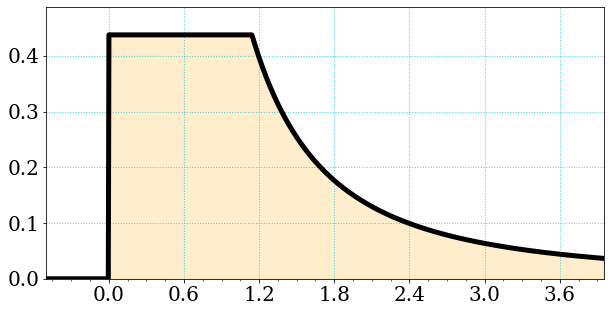
\includegraphics[width=0.9\textwidth]{2_53d22}
\end{figure}


3) вероятность равна:
$
\P(1,\!072\leqslant Z\leqslant 1,\!953)=
0,\!23843.
$



\item


%\folder 2_53d23.png
1) Функция распределения $F_Z(x)$ имеет вид:
$
F_Z(x)=\left\{
\begin{array}{l}
0, x\leqslant 0;\\
\frac{3 x}{20}, 0\leqslant x\leqslant \frac{10}{3}\approx 3,\!333;\\
1 - \frac{5}{3 x}, x\geqslant\frac{10}{3};
\end{array}.
\right.
$
2) Плотность распределения $f_Z(x)$ имеет вид:
$
f_Z(x)=\left\{
\begin{array}{l}
0, x<0;\\
\frac{3}{20}, 0\leqslant x\leqslant \frac{10}{3}\approx 3,\!333;\\
\frac{5}{3 x^{2}}, x\geqslant\frac{10}{3};
\end{array}.
\right.
$


\begin{figure}[H]
    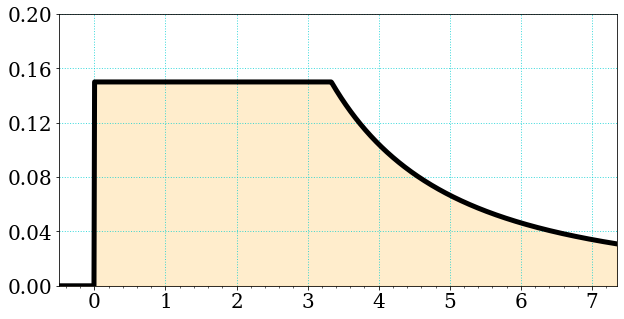
\includegraphics[width=0.9\textwidth]{2_53d23}
\end{figure}


3) вероятность равна:
$
\P(3,\!263\leqslant Z\leqslant 5,\!35)=
0,\!19897.
$



\item


%\folder 2_53d24.png
1) Функция распределения $F_Z(x)$ имеет вид:
$
F_Z(x)=\left\{
\begin{array}{l}
0, x\leqslant 0;\\
\frac{x}{8}, 0\leqslant x\leqslant 4\approx 4,\!0;\\
1 - \frac{2}{x}, x\geqslant4;
\end{array}.
\right.
$
2) Плотность распределения $f_Z(x)$ имеет вид:
$
f_Z(x)=\left\{
\begin{array}{l}
0, x<0;\\
\frac{1}{8}, 0\leqslant x\leqslant 4\approx 4,\!0;\\
\frac{2}{x^{2}}, x\geqslant4;
\end{array}.
\right.
$


\begin{figure}[H]
    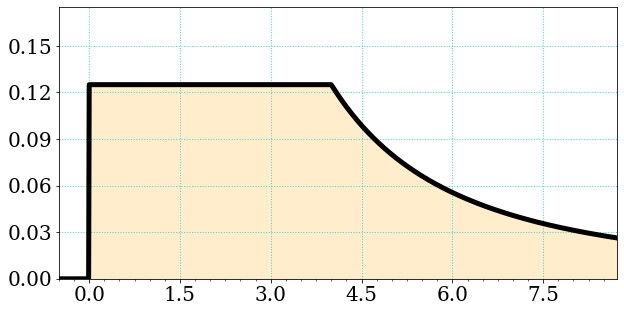
\includegraphics[width=0.9\textwidth]{2_53d24}
\end{figure}


3) вероятность равна:
$
\P(2,\!016\leqslant Z\leqslant 6,\!716)=
0,\!4502.
$



\item


%\folder 2_53d25.png
1) Функция распределения $F_Z(x)$ имеет вид:
$
F_Z(x)=\left\{
\begin{array}{l}
0, x\leqslant 0;\\
\frac{3 x}{10}, 0\leqslant x\leqslant \frac{5}{3}\approx 1,\!667;\\
1 - \frac{5}{6 x}, x\geqslant\frac{5}{3};
\end{array}.
\right.
$
2) Плотность распределения $f_Z(x)$ имеет вид:
$
f_Z(x)=\left\{
\begin{array}{l}
0, x<0;\\
\frac{3}{10}, 0\leqslant x\leqslant \frac{5}{3}\approx 1,\!667;\\
\frac{5}{6 x^{2}}, x\geqslant\frac{5}{3};
\end{array}.
\right.
$


\begin{figure}[H]
    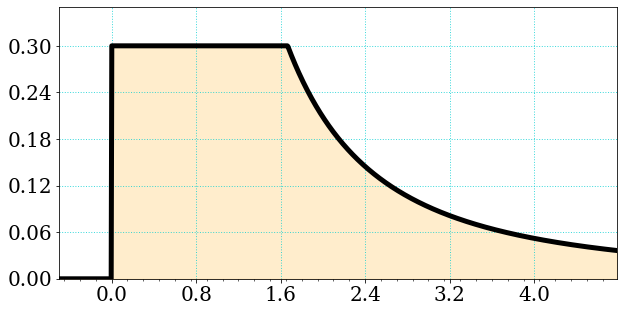
\includegraphics[width=0.9\textwidth]{2_53d25}
\end{figure}


3) вероятность равна:
$
\P(0,\!915\leqslant Z\leqslant 2,\!783)=
0,\!4261.
$



\item


Здесь сформулирована лемма Неймана-Пирсона в случае проверки двух простых гипотез. Тут же привдены
примеры построения наиболее мощного критерия.



\item


Тут ответы на все представленнные вопросы в данном вопросе



\item


Здесь формулировки критерия независимости Пирсона и приводится пример



\item


Найдём плотность рапределения как интеграл от ФР, а дальше всё и вовсе простою Ответ: $30155888444737842659$



\item


Найдём плотность рапределения как интеграл от ФР, а дальше всё и вовсе простою Ответ: $8000$



\item


Найдём плотность рапределения как интеграл от ФР, а дальше всё и вовсе простою Ответ: $30155888444737842659$



\item


Найдём плотность рапределения как интеграл от ФР, а дальше всё и вовсе простою Ответ: $8000$



\item


Найдём плотность рапределения как интеграл от ФР, а дальше всё и вовсе простою Ответ: $1174711139837$



\item


Найдём плотность рапределения как интеграл от ФР, а дальше всё и вовсе простою Ответ: $410338673$



\item


Найдём плотность рапределения как интеграл от ФР, а дальше всё и вовсе простою Ответ: $140608$



\item


Найдём плотность рапределения как интеграл от ФР, а дальше всё и вовсе простою Ответ: $308915776$



\item


Найдём плотность рапределения как интеграл от ФР, а дальше всё и вовсе простою Ответ: $782757789696$



\item


Найдём плотность рапределения как интеграл от ФР, а дальше всё и вовсе простою Ответ: $3936588805702081$



\item


Найдём плотность рапределения как интеграл от ФР, а дальше всё и вовсе простою Ответ: $6103515625$



\item


Найдём плотность рапределения как интеграл от ФР, а дальше всё и вовсе простою Ответ: $799006685782884121$



\item

	

	Первым этапом надо найти характеристики случайной величины $Y$

	$E(Y) = 10 * 0.24 + 7 * (1 - 0.24)$

	$Var(Y) = E(Y^2) - [E(Y)]^2 = 10^2 * 0.24 + 7^2 * (1 - 0.24) - [E(Y)]^2$


	Перейдем к рассмотрению характеристик условной случайно величины X

	$E(X) = E(E(X|Y)) = E[E(4 * Y) * 0.53 + E(9 * Y) * (1 - 0.53)] = E(Y) * (4 * 0.53 + 9 * (1 - 0.53)) = 49.022$

	$E(Var(X|Y)) = E[b * Var(c3 * Y) + (1 - b) * Var(c4 * Y)] = Var(Y) * (c3^2 * b + c4^2 * (1- b)) $

	$Var(E(X|Y)) = E(X^2|Y) - [E(X)]^2 = [E(Y)]^2 * (b * c3^2 + (1-b)*c4^2) - E(X)]^2$

	$Var(X) = E(Var(X|Y)) + Var(E(X|Y)) = 447.56552$
	


\item

	

	Первым этапом надо найти характеристики случайной величины $Y$

	$E(Y) = 1 * 0.7 + 10 * (1 - 0.7)$

	$Var(Y) = E(Y^2) - [E(Y)]^2 = 1^2 * 0.7 + 10^2 * (1 - 0.7) - [E(Y)]^2$


	Перейдем к рассмотрению характеристик условной случайно величины X

	$E(X) = E(E(X|Y)) = E[E(5 * Y) * 0.11 + E(8 * Y) * (1 - 0.11)] = E(Y) * (5 * 0.11 + 8 * (1 - 0.11)) = 28.379$

	$E(Var(X|Y)) = E[b * Var(c3 * Y) + (1 - b) * Var(c4 * Y)] = Var(Y) * (c3^2 * b + c4^2 * (1- b)) $

	$Var(E(X|Y)) = E(X^2|Y) - [E(X)]^2 = [E(Y)]^2 * (b * c3^2 + (1-b)*c4^2) - E(X)]^2$

	$Var(X) = E(Var(X|Y)) + Var(E(X|Y)) = 1027.72936$
	


\item

	

	Первым этапом надо найти характеристики случайной величины $Y$

	$E(Y) = 7 * 0.08 + 5 * (1 - 0.08)$

	$Var(Y) = E(Y^2) - [E(Y)]^2 = 7^2 * 0.08 + 5^2 * (1 - 0.08) - [E(Y)]^2$


	Перейдем к рассмотрению характеристик условной случайно величины X

	$E(X) = E(E(X|Y)) = E[E(9 * Y) * 0.24 + E(8 * Y) * (1 - 0.24)] = E(Y) * (9 * 0.24 + 8 * (1 - 0.24)) = 42.5184$

	$E(Var(X|Y)) = E[b * Var(c3 * Y) + (1 - b) * Var(c4 * Y)] = Var(Y) * (c3^2 * b + c4^2 * (1- b)) $

	$Var(E(X|Y)) = E(X^2|Y) - [E(X)]^2 = [E(Y)]^2 * (b * c3^2 + (1-b)*c4^2) - E(X)]^2$

	$Var(X) = E(Var(X|Y)) + Var(E(X|Y)) = 24.89926$
	


\item

	

	Первым этапом надо найти характеристики случайной величины $Y$

	$E(Y) = 2 * 0.61 + 1 * (1 - 0.61)$

	$Var(Y) = E(Y^2) - [E(Y)]^2 = 2^2 * 0.61 + 1^2 * (1 - 0.61) - [E(Y)]^2$


	Перейдем к рассмотрению характеристик условной случайно величины X

	$E(X) = E(E(X|Y)) = E[E(8 * Y) * 0.15 + E(6 * Y) * (1 - 0.15)] = E(Y) * (8 * 0.15 + 6 * (1 - 0.15)) = 10.143$

	$E(Var(X|Y)) = E[b * Var(c3 * Y) + (1 - b) * Var(c4 * Y)] = Var(Y) * (c3^2 * b + c4^2 * (1- b)) $

	$Var(E(X|Y)) = E(X^2|Y) - [E(X)]^2 = [E(Y)]^2 * (b * c3^2 + (1-b)*c4^2) - E(X)]^2$

	$Var(X) = E(Var(X|Y)) + Var(E(X|Y)) = 10.88555$
	


\item

	

	Первым этапом надо найти характеристики случайной величины $Y$

	$E(Y) = 3 * 0.33 + 4 * (1 - 0.33)$

	$Var(Y) = E(Y^2) - [E(Y)]^2 = 3^2 * 0.33 + 4^2 * (1 - 0.33) - [E(Y)]^2$


	Перейдем к рассмотрению характеристик условной случайно величины X

	$E(X) = E(E(X|Y)) = E[E(9 * Y) * 0.34 + E(7 * Y) * (1 - 0.34)] = E(Y) * (9 * 0.34 + 7 * (1 - 0.34)) = 28.1856$

	$E(Var(X|Y)) = E[b * Var(c3 * Y) + (1 - b) * Var(c4 * Y)] = Var(Y) * (c3^2 * b + c4^2 * (1- b)) $

	$Var(E(X|Y)) = E(X^2|Y) - [E(X)]^2 = [E(Y)]^2 * (b * c3^2 + (1-b)*c4^2) - E(X)]^2$

	$Var(X) = E(Var(X|Y)) + Var(E(X|Y)) = 25.32915$
	


\item

    
    Используя

	$E(X) = sum(X) / n$

	$Var(X) = E(X^2) - [E(X)]^2$

	$\mu_4(X) = E((X-E(X))^4)$

	$Ex = \frac{\mu_4(X)}{[\sigma(X)]^4} - 3$

	$r_{xy} = \frac{E(XY) - E(X) * E(Y)}{\sigma(X) * \sigma(Y)}$

    рассчитаем искомые значения.

    Ответы: $0.02724, 0.70603, 0.37291, -1.49926, 0.00012$.

    


\item

    
    Используя

	$E(X) = sum(X) / n$

	$Var(X) = E(X^2) - [E(X)]^2$

	$\mu_4(X) = E((X-E(X))^4)$

	$Ex = \frac{\mu_4(X)}{[\sigma(X)]^4} - 3$

	$r_{xy} = \frac{E(XY) - E(X) * E(Y)}{\sigma(X) * \sigma(Y)}$

    рассчитаем искомые значения.

    Ответы: $1.57801343872465 \cdot 10^{23}, 7.94364472492678 \cdot 10^{23}, 1.66305653632206 \cdot 10^{97}, 38.76647, 0.00352$.

    


\item

    
    Используя

	$E(X) = sum(X) / n$

	$Var(X) = E(X^2) - [E(X)]^2$

	$\mu_4(X) = E((X-E(X))^4)$

	$Ex = \frac{\mu_4(X)}{[\sigma(X)]^4} - 3$

	$r_{xy} = \frac{E(XY) - E(X) * E(Y)}{\sigma(X) * \sigma(Y)}$

    рассчитаем искомые значения.

    Ответы: $3.15966, 0.89438, 3.08587, 1.82265, -1.0 \cdot 10^{-5}$.

    


\item

    
    Используя

	$E(X) = sum(X) / n$

	$Var(X) = E(X^2) - [E(X)]^2$

	$\mu_4(X) = E((X-E(X))^4)$

	$Ex = \frac{\mu_4(X)}{[\sigma(X)]^4} - 3$

	$r_{xy} = \frac{E(XY) - E(X) * E(Y)}{\sigma(X) * \sigma(Y)}$

    рассчитаем искомые значения.

    Ответы: $1.53042524409691 \cdot 10^{35}, 9.46886335007349 \cdot 10^{35}, 5.07073544919377 \cdot 10^{145}, 60.07824, 0.00032$.

    


\item

    
    Используя

	$E(X) = sum(X) / n$

	$Var(X) = E(X^2) - [E(X)]^2$

	$\mu_4(X) = E((X-E(X))^4)$

	$Ex = \frac{\mu_4(X)}{[\sigma(X)]^4} - 3$

	$r_{xy} = \frac{E(XY) - E(X) * E(Y)}{\sigma(X) * \sigma(Y)}$

    рассчитаем искомые значения.

    Ответы: $-0.01464, 0.70686, 0.37349, -1.50394, 1.0 \cdot 10^{-5}$.

    


\item

    
    Используя

	$E(X) = sum(X) / n$

	$Var(X) = E(X^2) - [E(X)]^2$

	$\mu_4(X) = E((X-E(X))^4)$

	$Ex = \frac{\mu_4(X)}{[\sigma(X)]^4} - 3$

	$r_{xy} = \frac{E(XY) - E(X) * E(Y)}{\sigma(X) * \sigma(Y)}$

    рассчитаем искомые значения.

    Ответы: $4.25253870368928 \cdot 10^{41}, 2.85939246949767 \cdot 10^{42}, 4.98013632124489 \cdot 10^{171}, 71.49826, 0.00038$.

    


\item

    
    Используя

	$E(X) = sum(X) / n$

	$Var(X) = E(X^2) - [E(X)]^2$

	$\mu_4(X) = E((X-E(X))^4)$

	$Ex = \frac{\mu_4(X)}{[\sigma(X)]^4} - 3$

	$r_{xy} = \frac{E(XY) - E(X) * E(Y)}{\sigma(X) * \sigma(Y)}$

    рассчитаем искомые значения.

    Ответы: $5.66740783200168 \cdot 10^{31}, 3.33285124990578 \cdot 10^{32}, 7.03150966623892 \cdot 10^{131}, 53.98819, 0.0006$.

    


\item


1) Ковариация = $276.75$
2) Коэффициент корреляции = $1.373$



\item


1) Ковариация = $-518.0$
2) Коэффициент корреляции = $-2.6909$



\item


1) Ковариация = $-345.5$
2) Коэффициент корреляции = $-2.9554$



\item


1) Ковариация = $-350.8333$
2) Коэффициент корреляции = $-1.2925$



\item


1) Ковариация = $92.6667$
2) Коэффициент корреляции = $0.3814$



\item


1) Ковариация = $-876.6667$
2) Коэффициент корреляции = $-4.7659$



\item


1) Ковариация = $-126.3846$
2) Коэффициент корреляции = $-0.6429$



\item


1) Ковариация = $-335.0$
2) Коэффициент корреляции = $-2.4919$



\item


1) Ковариация = $-262.8$
2) Коэффициент корреляции = $-1.5753$



\item


1) Ковариация = $1210.3636$
2) Коэффициент корреляции = $5.5178$



\item

    


    k = len(marks) // k

    ex = np.sum([marks[m] * m for m in marks]) / n

    varx = np.var([ m for m in marks for temp in range(marks[m])]) / k * (n - k) / (n - 1)

    sigmax = varx**(0.5)
    Ответы: $9.83854, 0.99615$.

    


\item

    


    k = len(marks) // k

    ex = np.sum([marks[m] * m for m in marks]) / n

    varx = np.var([ m for m in marks for temp in range(marks[m])]) / k * (n - k) / (n - 1)

    sigmax = varx**(0.5)
    Ответы: $6.57937, 0.64259$.

    


\item

    


    k = len(marks) // k

    ex = np.sum([marks[m] * m for m in marks]) / n

    varx = np.var([ m for m in marks for temp in range(marks[m])]) / k * (n - k) / (n - 1)

    sigmax = varx**(0.5)
    Ответы: $6.14667, 0.65542$.

    


\item


1) математическое ожидание $\mathbb{E}(\bar Y)$: $3.85$ 
2) стандартное отклонение $\sigma(\bar X)$: $244.0153$
3) ковариацию $Cov(\bar X, \bar Y)$: $3.7764$



\item


1) математическое ожидание $\mathbb{E}(\bar Y)$: $3.6$ 
2) стандартное отклонение $\sigma(\bar X)$: $256.084$
3) ковариацию $Cov(\bar X, \bar Y)$: $-1.9911$



\item


1) математическое ожидание $\mathbb{E}(\bar Y)$: $3.6$ 
2) стандартное отклонение $\sigma(\bar X)$: $257.2355$
3) ковариацию $Cov(\bar X, \bar Y)$: $0.7091$



\item


1) математическое ожидание $\mathbb{E}(\bar Y)$: $3.75$ 
2) стандартное отклонение $\sigma(\bar X)$: $244.6913$
3) ковариацию $Cov(\bar X, \bar Y)$: $3.7904$



\item


1) математическое ожидание $\mathbb{E}(\bar Y)$: $4.16$ 
2) стандартное отклонение $\sigma(\bar X)$: $233.542$
3) ковариацию $Cov(\bar X, \bar Y)$: $0.4975$



\item


1) математическое ожидание $\mathbb{E}(\bar Y)$: $3.89$ 
2) стандартное отклонение $\sigma(\bar X)$: $239.4845$
3) ковариацию $Cov(\bar X, \bar Y)$: $0.3732$



\item


1) математическое ожидание $\mathbb{E}(\bar Y)$: $3.48$ 
2) стандартное отклонение $\sigma(\bar X)$: $256.5595$
3) ковариацию $Cov(\bar X, \bar Y)$: $0.5887$



\item


1) математическое ожидание $\mathbb{E}(\bar Y)$: $3.48$ 
2) стандартное отклонение $\sigma(\bar X)$: $248.8024$
3) ковариацию $Cov(\bar X, \bar Y)$: $2.0333$



\item


1) математическое ожидание $\mathbb{E}(\bar Y)$: $4.22$ 
2) стандартное отклонение $\sigma(\bar X)$: $255.4769$
3) ковариацию $Cov(\bar X, \bar Y)$: $-1.2655$



\item


1) математическое ожидание $\mathbb{E}(\bar Y)$: $3.59$ 
2) стандартное отклонение $\sigma(\bar X)$: $228.8693$
3) ковариацию $Cov(\bar X, \bar Y)$: $1.3324$



\item

    
        $E(Y|X+Y=1) = \frac{\sum(P(X=1 - y_i, y=y_i) * y_i)}{\sum(P(X=1 - y_i, y=y_i)}$.

        Ответ: $7.0893$
    


\item

    
        $E(Y|X+Y=1) = \frac{\sum(P(X=1 - y_i, y=y_i) * y_i)}{\sum(P(X=1 - y_i, y=y_i)}$.

        Ответ: $2.10982$
    


\item

    
        $E(Y|X+Y=1) = \frac{\sum(P(X=1 - y_i, y=y_i) * y_i)}{\sum(P(X=1 - y_i, y=y_i)}$.

        Ответ: $3.49618$
    


\item

    
        $E(Y|X+Y=1) = \frac{\sum(P(X=1 - y_i, y=y_i) * y_i)}{\sum(P(X=1 - y_i, y=y_i)}$.

        Ответ: $8.2921$
    


\item

    
        $E(Y|X+Y=1) = \frac{\sum(P(X=1 - y_i, y=y_i) * y_i)}{\sum(P(X=1 - y_i, y=y_i)}$.

        Ответ: $5.82286$
    


\item

    
        $E(Y|X+Y=1) = \frac{\sum(P(X=1 - y_i, y=y_i) * y_i)}{\sum(P(X=1 - y_i, y=y_i)}$.

        Ответ: $4.15479$
    


\item


Обе они несмещенные, потому что в числителе выходит в сумме 10.
Какая-то точно должна быть, а может и нет....



\item


Обе они несмещенные, потому что в числителе выходит в сумме 10.
Какая-то точно должна быть, а может и нет....



\item


Обе они несмещенные, потому что в числителе выходит в сумме 10.
Какая-то точно должна быть, а может и нет....



\item


Обе они несмещенные, потому что в числителе выходит в сумме 10.
Какая-то точно должна быть, а может и нет....



\item


Обе они несмещенные, потому что в числителе выходит в сумме 10.
Какая-то точно должна быть, а может и нет....



\item


Обе они несмещенные, потому что в числителе выходит в сумме 10.
Какая-то точно должна быть, а может и нет....



\item


Обе они несмещенные, потому что в числителе выходит в сумме 10.
Какая-то точно должна быть, а может и нет....



\item


Обе они несмещенные, потому что в числителе выходит в сумме 10.
Какая-то точно должна быть, а может и нет....



\item


Обе они несмещенные, потому что в числителе выходит в сумме 10.
Какая-то точно должна быть, а может и нет....



\item


Обе они несмещенные, потому что в числителе выходит в сумме 10.
Какая-то точно должна быть, а может и нет....



\item

	

	$f(x) = F'(x) = \beta \cdot x^{\beta - 1}$

	$\mu_{1} = E(X) = \int_{-\inf}^{\inf}x \cdot f(x) = \int_{-\inf}^{\inf} \beta \cdot x^{\beta} = \beta \cdot \frac{x^{\beta + 1}}{\beta + 1}\bigg|_0^1 = \frac{\beta}{\beta + 1}$

	$\beta = (\beta + 1) \cdot 60.0$

	$\beta = \frac{60.0}{1 - 60.0}$

	$ P(x \le 52.0) = F(52.0) = 52.0^{1.5} $

    Ответ: $1.5, 0.37$
	


\item

	

	$f(x) = F'(x) = \beta \cdot x^{\beta - 1}$

	$\mu_{1} = E(X) = \int_{-\inf}^{\inf}x \cdot f(x) = \int_{-\inf}^{\inf} \beta \cdot x^{\beta} = \beta \cdot \frac{x^{\beta + 1}}{\beta + 1}\bigg|_0^1 = \frac{\beta}{\beta + 1}$

	$\beta = (\beta + 1) \cdot 71.0$

	$\beta = \frac{71.0}{1 - 71.0}$

	$ P(x \le 62.0) = F(62.0) = 62.0^{2.45} $

    Ответ: $2.45, 0.31$
	


\item

	

	$f(x) = F'(x) = \beta \cdot x^{\beta - 1}$

	$\mu_{1} = E(X) = \int_{-\inf}^{\inf}x \cdot f(x) = \int_{-\inf}^{\inf} \beta \cdot x^{\beta} = \beta \cdot \frac{x^{\beta + 1}}{\beta + 1}\bigg|_0^1 = \frac{\beta}{\beta + 1}$

	$\beta = (\beta + 1) \cdot 67.0$

	$\beta = \frac{67.0}{1 - 67.0}$

	$ P(x \le 52.0) = F(52.0) = 52.0^{2.03} $

    Ответ: $2.03, 0.27$
	


\item

	

	$f(x) = F'(x) = \beta \cdot x^{\beta - 1}$

	$\mu_{1} = E(X) = \int_{-\inf}^{\inf}x \cdot f(x) = \int_{-\inf}^{\inf} \beta \cdot x^{\beta} = \beta \cdot \frac{x^{\beta + 1}}{\beta + 1}\bigg|_0^1 = \frac{\beta}{\beta + 1}$

	$\beta = (\beta + 1) \cdot 55.0$

	$\beta = \frac{55.0}{1 - 55.0}$

	$ P(x \le 50.0) = F(50.0) = 50.0^{1.22} $

    Ответ: $1.22, 0.43$
	


\item

	

	$f(x) = F'(x) = \beta \cdot x^{\beta - 1}$

	$\mu_{1} = E(X) = \int_{-\inf}^{\inf}x \cdot f(x) = \int_{-\inf}^{\inf} \beta \cdot x^{\beta} = \beta \cdot \frac{x^{\beta + 1}}{\beta + 1}\bigg|_0^1 = \frac{\beta}{\beta + 1}$

	$\beta = (\beta + 1) \cdot 62.0$

	$\beta = \frac{62.0}{1 - 62.0}$

	$ P(x \le 59.0) = F(59.0) = 59.0^{1.63} $

    Ответ: $1.63, 0.42$
	


\item

	

	$f(x) = F'(x) = \beta \cdot x^{\beta - 1}$

	$\mu_{1} = E(X) = \int_{-\inf}^{\inf}x \cdot f(x) = \int_{-\inf}^{\inf} \beta \cdot x^{\beta} = \beta \cdot \frac{x^{\beta + 1}}{\beta + 1}\bigg|_0^1 = \frac{\beta}{\beta + 1}$

	$\beta = (\beta + 1) \cdot 74.0$

	$\beta = \frac{74.0}{1 - 74.0}$

	$ P(x \le 73.0) = F(73.0) = 73.0^{2.85} $

    Ответ: $2.85, 0.41$
	


\item

	

	$f(x) = F'(x) = \beta \cdot x^{\beta - 1}$

	$\mu_{1} = E(X) = \int_{-\inf}^{\inf}x \cdot f(x) = \int_{-\inf}^{\inf} \beta \cdot x^{\beta} = \beta \cdot \frac{x^{\beta + 1}}{\beta + 1}\bigg|_0^1 = \frac{\beta}{\beta + 1}$

	$\beta = (\beta + 1) \cdot 76.0$

	$\beta = \frac{76.0}{1 - 76.0}$

	$ P(x \le 74.0) = F(74.0) = 74.0^{3.17} $

    Ответ: $3.17, 0.39$
	


\item

	

	$f(x) = F'(x) = \beta \cdot x^{\beta - 1}$

	$\mu_{1} = E(X) = \int_{-\inf}^{\inf}x \cdot f(x) = \int_{-\inf}^{\inf} \beta \cdot x^{\beta} = \beta \cdot \frac{x^{\beta + 1}}{\beta + 1}\bigg|_0^1 = \frac{\beta}{\beta + 1}$

	$\beta = (\beta + 1) \cdot 57.0$

	$\beta = \frac{57.0}{1 - 57.0}$

	$ P(x \le 51.0) = F(51.0) = 51.0^{1.33} $

    Ответ: $1.33, 0.41$
	


\end{enumerate}
\end{document}